\subsection{Complexes of A-modules}

DEFINITION 1. --- A differential complex of A-modules is a pair (C, d) consisting of a graded A-module C and an endomorphism \(d: \mathbf{C} \to \mathbf{C}\) graded of descending degree -1 and such that \(d \circ d = 0\) .

It is also called a complex of A-modules, or an A-complex, or simply a complex. One often writes C instead of (C, d); the endomorphism d is called the differential of the complex (C, d), or, by abuse of language, of C.

If \(C_{n}\) (resp. \(C^{n}\) ) is the homogeneous component of descending (resp. ascending) degree n of C, the datum of d is equivalent to that of the sequence of homomorphisms

\[
\dots \longrightarrow \mathrm{C} _ {n + 1} \xrightarrow {d _ {n + 1}} \mathrm{C} _ {n} \xrightarrow {d _ {n}} \mathrm{C} _ {n - 1} \longrightarrow \dots\tag{1}
\]

resp.

\[
\dots \longrightarrow \mathrm{C} ^ {n - 1} \xrightarrow {d ^ {n - 1}} \mathrm{C} ^ {n} \xrightarrow {d ^ {n}} \mathrm{C} ^ {n + 1} \longrightarrow \dots\tag{1'}
\]

such that \(d_n \circ d_{n+1} = 0\) for all \(n \in \mathbf{Z}\) (resp. \(d^n \circ d^{n-1} = 0\) for all \(n \in \mathbf{Z}\) ). By abuse of language, the datum of such a sequence of A-modules and homomorphisms will also be called a complex.

As a mnemonic, note that when one "follows the direction of the arrows" in diagrams (1) and (1'), the descending degree decreases and the ascending degree increases.

Every graded A-module will tacitly be regarded as a complex by equipping it with the zero differential; the complexes thus obtained will be called complexes with zero differential. In particular, every A-module M will be endowed with the unique structure of an A-complex such that \(M_{0} = M^{0} = M\) . The complex (C, d) is said to be zero if C is reduced to 0. In what follows, we denote by 0 a zero complex, chosen once and for all.

Let us adjoin to the ordered set Z two elements denoted \(-\infty\) and \(+\infty\) ; denote by \(\overline{Z}\) the set obtained, and endow it with the order relation extending that of Z and such that \(-\infty < n < +\infty\) for all \(n \in Z\) ; every subset of \(\overline{Z}\) has a lower bound and an upper bound.

Let C be a complex; the right and left bounds \(^{1}\) of C are the elements \(b_{d}(\mathbf{C})\) and \(b_{g}(\mathbf{C})\) of \(\overline{\mathbf{Z}}\) defined by

\[
b _ {d} (\mathbf {C}) = \inf \left\{n \in \mathbf {Z}, \mathrm{C} _ {n} \neq 0 \right\}, \quad b _ {g} (\mathbf {C}) = \sup \left\{n \in \mathbf {Z}, \mathrm{C} _ {n} \neq 0 \right\}.
\]

One says that C is zero on the right if \(b_{d}(\mathbf{C}) \geqslant 0\) , bounded on the right if \(b_{d}(\mathbf{C}) \neq -\infty\) , zero on the left if \(b_{g}(\mathbf{C}) \leqslant 0\) , bounded on the left if \(b_{g}(\mathbf{C}) \neq +\infty\) ; one says that C is bounded if

\[
b _ {d} (\mathbf {C}) \neq - \infty , \quad b _ {g} (\mathbf {C}) \neq + \infty .
\]

The length \(^{2}\) of C, denoted by \(l(\mathbf{C})\), is the element of \(\overline{\mathbf{Z}}\) defined as follows: if C is zero, \(l(\mathbf{C}) = -\infty\) ; if C is bounded and nonzero \(l(\mathbf{C}) = b_{g}(\mathbf{C}) - b_{d}(\mathbf{C})\) ; if C is not bounded, \(l(\mathbf{C}) = +\infty\) . * With the conventions of TG, IV, p.~13-17, one always has \(l(\mathbf{C}) = b_{g}(\mathbf{C}) - b_{d}(\mathbf{C})\) . *

For example, if \(k\) consecutive components of \(C\) are nonzero, the others being zero, we have \(l(C) = k - 1\) if \(k > 0\) , \(l(C) = -\infty\) if \(k = 0\) .

We say that the complex (C, d) is free, projective, flat, injective, if each of the modules \(C_{n}\) is so. Note that the complex (C, d) is projective or flat if and only if the module C is (II, p.~39, prop. 3 and X, p.~8, prop. 4), but C can be free without the complex (C, d) being so (since a direct summand of a free module is not always free), just as (C, d) can be injective without C being so (X, p.~170, exercise 21).

\pandocbounded{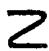
\includegraphics[keepaspectratio]{images/part001_579990b7.jpg}}

Let (C, d) be a complex. We set \(\mathbf{Z}(\mathbf{C}, d) = \operatorname{Ker}(d)\) , \(\mathbf{B}(\mathbf{C}, d) = \operatorname{Im}(d)\) ; these are graded submodules of C, called respectively the module of cycles and the module of boundaries of (C, d); the homogeneous components of \(\mathbf{Z}(\mathbf{C}, d)\) and \(\mathbf{B}(\mathbf{C}, d)\) are denoted \(\mathbf{Z}_{n}(\mathbf{C}, d) = \mathbf{Z}^{-n}(\mathbf{C}, d)\) , \(\mathbf{B}_{n}(\mathbf{C}, d) = \mathbf{B}^{-n}(\mathbf{C}, d)\) ; we have \(\mathbf{Z}_{n}(\mathbf{C}, d) = \operatorname{Ker}(d_{n})\) , \(\mathbf{B}_{n}(\mathbf{C}, d) = \operatorname{Im}(d_{n+1})\) , \(\mathbf{Z}^{n}(\mathbf{C}, d) = \operatorname{Ker}(d^{n})\) , \(\mathbf{B}^{n}(\mathbf{C}, d) = \operatorname{Im}(d^{n-1})\) .

Since \(d \circ d = 0\) , we have \(\mathrm{B}(\mathrm{C}) \subset \mathrm{Z}(\mathrm{C})\) ; two cycles are said to be homologous if their difference is a boundary; the quotient graded module \(\mathrm{H}(\mathrm{C}, d) = \mathrm{Z}(\mathrm{C}, d)/\mathrm{B}(\mathrm{C}, d)\) is called the homology module of \((\mathrm{C}, d)\) ; its elements are the homology classes; its homogeneous components are denoted \(\mathrm{H}_n(\mathrm{C}, d) = \mathrm{H}^{-n}(\mathrm{C}, d)\) .

Example. --- If C has zero differential, we have \(Z(C) = C\) , \(B(C) = 0\) and \(H(C)\) is canonically identified with \(C\) .

We have exact sequences, called canonical:

\((I_{n})\)

\[
0 \longrightarrow \mathrm{Z} _ {n} (\mathrm{C}) \longrightarrow \mathrm{C} _ {n} \stackrel {\delta_ {n}} {\longrightarrow} \mathrm{B} _ {n - 1} (\mathrm{C}) \longrightarrow 0\tag{\((\mathrm{II}_{n})\)}
\]

\[
0 \longrightarrow \mathrm{B} _ {n} (\mathrm{C}) \longrightarrow \mathrm{Z} _ {n} (\mathrm{C}) \longrightarrow \mathrm{H} _ {n} (\mathrm{C}) \longrightarrow 0
\]

\((\mathrm{III}_{n})\)

\[
0 \longrightarrow \mathrm{B} _ {n} (\mathrm{C}) \longrightarrow \mathrm{C} _ {n} \longrightarrow \mathrm{C} _ {n} / \mathrm{B} _ {n} (\mathrm{C}) \longrightarrow 0
\]

\((\mathrm{IV}_n)\)

\[
0 \longrightarrow \mathrm{H} _ {n} (\mathrm{C}) \longrightarrow \mathrm{C} _ {n} / \mathrm{B} _ {n} (\mathrm{C}) \stackrel {\overline {{\delta}} _ {n}} {\longrightarrow} \mathrm{B} _ {n - 1} (\mathrm{C}) \longrightarrow 0
\]

where \(\delta_{n}\) and \(\overline{\delta}_{n}\) are deduced from \(d_{n}\) . By combining \((\mathrm{IV}_{n})\) and \((\mathrm{II}_{n-1})\) , one obtains the exact sequence

\[
0 \rightarrow \mathrm{H} _ {n} (\mathrm{C}) \rightarrow \mathrm{C} _ {n} / \mathrm{B} _ {n} (\mathrm{C}) \rightarrow \mathrm{Z} _ {n - 1} (\mathrm{C}) \rightarrow \mathrm{H} _ {n - 1} (\mathrm{C}) \rightarrow 0,\tag{\((\mathbf{V}_n)\)}
\]

which is also written, changing n to -n

\[
0 \rightarrow \mathrm{H} ^ {n} (\mathrm{C}) \rightarrow \mathrm{C} ^ {n} / \mathrm{B} ^ {n} (\mathrm{C}) \rightarrow \mathrm{Z} ^ {n + 1} (\mathrm{C}) \rightarrow , \mathrm{H} ^ {n + 1} (\mathrm{C}) \rightarrow 0.\tag{\((\mathbf{V}^n)\)}
\]

DEFINITION 2. --- Let (C, d) and (C', d') be two complexes. A morphism \(^{1}\) from (C, d) to (C', d') is a graded A-homomorphism u of degree 0 from C to C' such that

\[
d ^ {\prime} \circ u = u \circ d.
\]

For every \(n\) we therefore have \(d_n' \circ u_n = u_{n-1} \circ d_n\) and \(d''n \circ u^n = u^{n+1} \circ d^n\) . We have

\[
u (\mathbf {Z} (\mathbf {C})) \subset \mathbf {Z} (\mathbf {C} ^ {\prime}), \quad u (\mathbf {B} (\mathbf {C})) \subset \mathbf {B} (\mathbf {C} ^ {\prime}),
\]

and we denote by \(Z(u):Z(C)\to Z(C')\) , \(B(u):B(C)\to B(C')\) , \(H(u):H(C)\to H(C')\) the homomorphisms of A-modules deduced from them; the homogeneous components of these morphisms are denoted \(Z_{n}(u)\) , \(Z^{n}(u)\) , \ldots{}

If \(v\) is another morphism of \((\mathbf{C}, d)\) to \((\mathbf{C}', d')\) , then \(u + v\) is a morphism of \((\mathbf{C}, d)\) to \((\mathbf{C}', d')\) , and we have

\[
\mathbf {Z} (u + v) = \mathbf {Z} (u) + \mathbf {Z} (v), \quad \mathbf {B} (u + v) = \mathbf {B} (u) + \mathbf {B} (v), \quad \mathbf {H} (u + v) = \mathbf {H} (u) + \mathbf {H} (v)
\]

Similarly, if A is an algebra over a commutative ring \(k\) , and if \(\lambda \in k\) , then \(\lambda u\) is a morphism of \((C, d)\) to \((C', d')\) and we have

\[
\mathbf {Z} (\lambda u) = \lambda \mathbf {Z} (u), \quad \mathbf {B} (\lambda u) = \lambda \mathbf {B} (u), \quad \mathbf {H} (\lambda u) = \lambda \mathbf {H} (u).
\]

If \(u': (C', d') \to (C'', d'')\) is another morphism of complexes, then \(u' \circ u\) is a morphism of \((C, d)\) to \((C'', d'')\) and we have

\[
\mathrm{Z} \left(u ^ {\prime} \circ u\right) = \mathrm{Z} \left(u ^ {\prime}\right) \circ \mathrm{Z} (u), \quad \mathrm{B} \left(u ^ {\prime} \circ u\right) = \mathrm{B} \left(u ^ {\prime}\right) \circ \mathrm{B} (u), \quad \mathrm{H} \left(u ^ {\prime} \circ u\right) = \mathrm{H} \left(u ^ {\prime}\right) \circ \mathrm{H} (u).
\]

It is clear that a bijective morphism is an isomorphism.

DEFINITION 3. --- Let (C, d) and (C', d') be two complexes. A homology morphism (or quasi-isomorphism) from (C, d) to (C', d') is a morphism u from (C, d) to (C', d') such that H(u) is bijective.

Every isomorphism is a homology morphism, and every morphism composed of homology morphisms is a homology morphism.

One says that (C, d) has zero homology if H(C) = 0, that is, if the unique morphism of complexes \(0 \rightarrow C\) (resp. C → 0) is a homology morphism. One says that (C, d) is acyclic in descending degree n (resp. in ascending degree n) if \(\mathrm{H}_{n}(\mathrm{C}) = 0\) (resp. \(\mathrm{H}^{n}(\mathrm{C}) = 0\) ).

Let (C, d) be a complex and \(p \in Z\) . The p-th translate of (C, d) is the complex (C(p), d(p)) obtained as follows: C(p) is the A-module obtained by shifting the grading of C by p (II, p.~163; example 3), so that

\[
\mathrm{C} (p) _ {n} = \mathrm{C} _ {n + p}, \quad \mathrm{C} (p) ^ {n} = \mathrm{C} ^ {n - p};
\]

in particular \(\mathbf{C}(p)_{0} = \mathbf{C}_{p}\) ; one also notes that C is the direct sum of its graded submodules \(\mathbf{C}_{p}(-p)\) , \(p \in \mathbf{Z}\) (resp. \(\mathbf{C}^{p}(p)\) , \(p \in \mathbf{Z}\) ). One sets \(d(p) = (-1)^{p} d\) . We have \(\mathbf{Z}(\mathbf{C}(p)) = \mathbf{Z}(\mathbf{C})(p)\) , \(\mathbf{B}(\mathbf{C}(p)) = \mathbf{B}(\mathbf{C})(p)\) and \(\mathrm{H}(\mathbf{C}(p)) = \mathrm{H}(\mathbf{C})(p)\) .

For example, \(d\) is a morphism of complexes from C to C(-1) and

\[
\mathrm{H} (d): \mathrm{H} (\mathbf {C}) \to \mathrm{H} (\mathbf {C}) (- 1)
\]

is zero.

For every morphism of complexes \(u:(\mathbf{C},d)\to(\mathbf{C}^{\prime},d^{\prime})\) , and every \(p\in\mathbf{Z}\) , \(u\) is also a morphism of \((\mathbf{C}(p),d(p))\) to \((\mathbf{C}^{\prime}(p),d^{\prime}(p))\) ; it is sometimes denoted \(u(p)\) and we have

\[
u (p) _ {n} = u _ {n + p}, \quad u (p) ^ {n} = u ^ {n - p}.
\]
% semantic-fragments: legacy-input-seam
\relax{}
